\documentclass[12pt, a4paper]{report}
%\usepackage{tgtermes} % for times romans font
\usepackage{float}
\usepackage{natbib}
\usepackage{amsmath}
\usepackage{comment}
\usepackage{graphicx}
\usepackage{etoolbox}
\usepackage{geometry}
\usepackage{fancyhdr}
\usepackage{amsfonts}
\usepackage{tocbibind} % adds 'Contents' to TOC
\usepackage[T1]{fontenc}
\usepackage[utf8]{inputenc} % use utf8x if utf8 causes error
\usepackage[UKenglish]{babel}
\usepackage[section]{placeins}
\usepackage[dvipsnames]{xcolor}
\usepackage[pdftex, pdfauthor={Jovial Joe Jayarson}, pdftitle={OpenAI GPT-3}, pdfsubject={Language Model - Seminar Report}]{hyperref}

%\usepackage{tgtermes} % for times romans font
\usepackage{float}
\usepackage{natbib}
\usepackage{xpatch}
\usepackage{amsmath}
\usepackage{comment}
\usepackage{graphicx}
\usepackage{etoolbox}
\usepackage{geometry}
\usepackage{fancyhdr}
\usepackage{setspace}
\usepackage{amsfonts}
\usepackage{blindtext}
\usepackage{tocbibind} % adds 'Contents' to TOC
\usepackage[T1]{fontenc}
\usepackage[utf8]{inputenc} % use utf8x if utf8 causes error
\usepackage[UKenglish]{babel}
\usepackage[section]{placeins}
\usepackage[dvipsnames]{xcolor}
\usepackage[useregional]{datetime2}
\usepackage[pdftex, pdfauthor={Jovial Joe Jayarson}, pdftitle={OpenAI GPT-3}, pdfsubject={Language Model - Seminar Report}]{hyperref}

\newcommand{\mydate}{\DTMdisplaydate{2020}{12}{05}{-1}}

\hypersetup{
    colorlinks      = true,
    urlcolor        = gray,
    linkcolor       = magenta,
    citecolor       = brown,
    citebordercolor = green,
    urlbordercolor  = white,
    linkbordercolor = blue,
}

\graphicspath{{../images/}}
\setlength{\headheight}{32pt}
%\setcitestyle{open={},close={},numbers}
\AtBeginDocument{\hypersetup{pdfborder={0 0 1}}}
\AtBeginEnvironment{quote}{\singlespacing\small}

\title{\textbf{OpenAI GPT-3} \\ \vspace{1cm} \large A seminar report during 2020 - 2021, \\ submitted to APJ Abdul Kalam Technological University in partial fulfillment of the requirements for the award of the degree of \\ \vspace{0.5cm} \large \textbf{Bachelor of Technology \\ in \\ Computer Science and Engineering} \\ \vspace{0.5cm} \large by}
\author{\textbf{Jovial Joe Jayarson (IES17CS016)}}
\date{}

%>>>>>>>>>>>>>>>>>>>>>>> Header & Footer >>>>>>>>>>>>>>>>>>>>>>>
\makeatletter
\patchcmd{\f@nch@head}{\rlap}{\color{gray}\rlap}{}{}
%\patchcmd{\headrule}{\hrule}{\color{gray}\hrule}{}{}
\patchcmd{\f@nch@foot}{\rlap}{\color{gray}\rlap}{}{}
%\patchcmd{\footrule}{\hrule}{\color{gray}\hrule}{}{}

\xpatchcmd{\@makeschapterhead}{%
  \Huge \bfseries  #1\par\nobreak%
}{%
  \Huge \bfseries\centering #1\par\nobreak%
}{\typeout{Patched makeschapterhead}}{\typeout{patching of @makeschapterhead failed}}


\xpatchcmd{\@makechapterhead}{%
  \huge\bfseries \@chapapp\space \thechapter
}{%
  \huge\bfseries\centering \@chapapp\space \thechapter
}{\typeout{Patched @makechapterhead}}{\typeout{Patching of @makechapterhead failed}}

\makeatother

\pagestyle{fancy}
\fancyhf{}
\lhead{Department of CSE}
\rhead{Seminar Report 2020-21}
\cfoot{\thepage}
\rfoot{IES College of Engineering}
\renewcommand{\headrulewidth}{0pt}
\renewcommand{\footrulewidth}{0pt}
%<<<<<<<<<<<<<<<<<<<<<<< Header & Footer <<<<<<<<<<<<<<<<<<<<<<<

%#################################################################
%                      Document Begins Here                      %
%#################################################################

\begin{document}

\newgeometry{left=3cm,right=3cm,top=3cm,bottom=3cm}

\makeatletter
\thispagestyle{empty}
\begin{titlepage}
    \begin{center}
        \vspace*{\fill}
        {\huge \@title }\\[0.5cm]
        {\@author} \\[0.5cm]
        {\@date}\\[10ex]
        
\includegraphics[width=0.5\linewidth]{iesce.png}\\[10ex]
        {\large Department of Computer Science and Engineering \\ \textbf{IES College of Engineering, Chittilappilly - 680551}}
        \vspace*{\fill}
    \end{center}
\end{titlepage}

\pagenumbering{roman}

\newpage
\thispagestyle{plain}
\vspace*{\fill}
\begin{center}
    \textbf{\textsc{IES College of Engineering}}\\[0.5cm]
    \textbf{\textsc{Department of Computer Science and Engineering}}\\[1cm]
    
\includegraphics{iesce.png}
    \section*{Certificate}
    \addcontentsline{toc}{chapter}{Certificate}
    This is to certify that the seminar report entitled \\[0.3cm] \textbf{\large Open AI GPT-3} \\[0.3cm] submitted by \\[0.3cm] \textbf{Jovial Joe Jayarson} \\[0.3cm] in partial fulfilment of the requirements of the degree of \emph{Bachelor of Technology in Computer Science and Engineering}, to APJ Abdul Kalam Technological University is a record of \emph{bona fide}  work done by him under my supervision and guidance and this work has not been submitted elsewhere for any degree or diploma. \\[2cm]
\end{center}

\begin{table}[h]
    \centering
    \begin{tabular}{ l l c c }
                        &          & \rule{4.5cm}{0.15mm}     & \rule{4.5cm}{0.15mm}     \\
        \textbf{Place}: & Thrissur & \textbf{Ms. Shejina N M} & \textbf{Dr. Kiruthiga G} \\
                        &          & Asst. Professor, CSE     & Head of the Department   \\
        \textbf{Date}:  &          & (Seminar Coordinator)    & CSE                      \\
    \end{tabular}
\end{table}
\vspace*{\fill}
\newpage
\vspace*{\fill}
\begin{center}
    \section*{Acknowledgement}
    \addcontentsline{toc}{chapter}{Acknowledgements}
\end{center}

I'm excited as I present this report on \emph{Open AI GPT-3} as part of the final year B.Tech Computer Science and Engineering seminar. Allow me to take this opportunity to first thank the God Almighty for providing His grace and guidance in this dispensation.

Sincere thanks to \emph{Dr. Brilly S Sangeetha}, Principal, for providing all the required facilities to make this a great success. I acknowledge, with all respect, the encouraging presence of \emph{Dr. Kriuthiga G}, Head of the Department, all along the way. I stand with unspeakable gratitude to my guide \emph{Mr. Ebin P M}, Assistant Professor, for his motivation, attention, and support all time.

Last but not the least, I convey my warm regards to all the well wishers, family members and friends who have helped me during needed times.

\vspace{0.5em}
\begin{center}
    May God bless us all.
\end{center}
\vspace*{\fill}
\newpage
\vspace*{\fill}
\begin{center}
    \section*{Abstract}
    \addcontentsline{toc}{chapter}{Abstract}
\end{center}
The word `GPT-3' has brought the tech world to an unspoken frenzy. It seems to keep on appearing over and over again, all across the technical media corpus. GPT-3 stands for Generative Pre-trained Transformer, which is a language model, created by the engineers at OpenAI. A language model takes in sequences of text input and spits out another sequence of coherent text, which is in some way related to the input. Parameters in a machine learning models can be thought of as knobs and dials of a function which are continuously tweaked until an optimal desired response is obtained from the model. This model in massive, in the sense that it has huge number of these parameters. Even more interesting is its incredible capability to generate coherent literature. The media is hyped with the mind boggling, selected results of GPT-3. The report aims to delves deep into GPT-3 to realize its architecture and how it works. To be unbiased, this report also explores what some of the critiques has voiced. Finally it concludes with certain interesting remarks on GPT-3.
\vspace*{\fill}

{
    \hypersetup{hidelinks}

    \tableofcontents
    \thispagestyle{fancy}

    \listoffigures
    \thispagestyle{fancy}

    %\listoftables
    %\thispagestyle{fancy}
}

\chapter*{Introduction}
\label{chap:introduction}
\thispagestyle{fancy}
\pagenumbering{arabic}
\addcontentsline{toc}{chapter}{\nameref{chap:introduction}}

\hspace{0.5cm} Generative Pre-trained Transformer 3 (GPT-3) is an autoregressive language model that uses deep learning to produce human-like text. It is the third-generation language prediction model in the GPT-n series created by OpenAI\cite{wiki:gpt3}. A May 28, 2020 arXiv preprint by a group of 31 engineers and researchers at OpenAI, described the development of GPT-3, a third-generation ``state-of-the-art language model''. In his July 29, 2020 review in The New York Times, Farhad Manjoo said that GPT-3 - which can generate computer code and poetry, as well as prose - is not just `amazing', `spooky', and `humbling', but also `more than a little terrifying'\cite{art:hhwt}.

GPT-3's full version has a capacity of 175 billion machine learning parameters. GPT-3, which was introduced in May 2020, and is in beta testing as of July 2020\cite{art:wtla}. One architecture used in natural language processing (NLP) is a neural network based on a deep learning model that was first introduced in 2017 - the Transformer\cite{2017arXiv170603762V}. GPT-3's higher number of parameters grants it a paramount level of accuracy relative to previous versions with smaller capacity. GPT-3's capacity is ten times larger than that of Microsoft's Turing NLG. On June 11, 2020, OpenAI announced that users could request access to its user-friendly GPT-3 API - a ``machine learning toolset'' - to help OpenAI `explore the strengths and limits' of this new technology.

The invitation described how this API had a general-purpose `text in, text out' interface that can complete almost any English language task, instead of the usual single use-case. GPT-3's mind-boggling performance has convinced many that super-intelligence is closer than we think - or at least, that AI-generated code is closer than we think. It generates creative, insightful, deep, and even breathtakingly beautiful content\cite{art:wtla}.
\vspace*{\fill}

%>>>>>>>>>>>>>>>>>>>>>>> Literature >>>>>>>>>>>>>>>>>>>>>>>
%\chapter*{Literature Survey}
%\label{chap:literature}
%\addcontentsline{toc}{chapter}{\nameref{chap:literature}}
%<<<<<<<<<<<<<<<<<<<<<<< Literature <<<<<<<<<<<<<<<<<<<<<<<

\chapter*{Overview of GPT}
\label{chap:overview}
\thispagestyle{fancy}
\addcontentsline{toc}{chapter}{\nameref{chap:overview}}

\hspace{0.5cm} OpenAI is an artificial intelligence research laboratory. The organization was founded in San Francisco in late 2015 by Elon Musk, Sam Altman, and others. June 11, 2018 - Alec Radford and colleagues, and published initial GPT in preprint on OpenAI's website. 

\subsubsection*{Generative Models}
\label{subsub:genmodls}

\hspace{0.5cm} Those language models which generate a coherent output from natural language given as input are called generative models. Open AI published the following versions of GPT from 2018-20

\begin{itemize}
    \item GPT : Was published in preprint on OpenAI's website on June 11, 2018. It shows how a generative model of language is able to acquire world knowledge. It could process long-range dependencies. Was pre-trained on a diverse corpus with long stretches of contiguous text.
    \item GPT-2 : Is an unsupervised transformer language model and successor to GPT which was first announced in February 2019. It's full version has around 1.5B parameters. It achieves state-of-the-art accuracy and perplexity on 7 of 8 zero-shot tasks.
    \item GPT-3 : Is an autoregressive language model and successor to GPT-2 which was showcased in May 2020. The full version of GPT-3 contains 175B parameters. Pre-training GPT-3 required several thousand petaflop/s-days of compute. On September 23, 2020, GPT-3 was licensed exclusively to Microsoft.
\end{itemize}

\begin{figure}[!htbp]
    \centering
    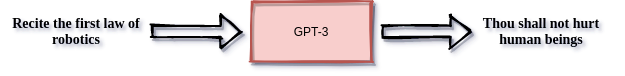
\includegraphics[width=0.9\textwidth]{gpt3.png}
    \caption[GPT-3 Overview]{GPT-3 Overview}
    \label{fig:gpt3ovrviw}
\end{figure}

\vspace*{\fill}

\chapter*{Prerequisites to GPT-3}
\label{chap:prereq}
\thispagestyle{fancy}
\addcontentsline{toc}{chapter}{\nameref{chap:prereq}}

\hspace{0.5cm} This seminar covers advanced topics under artificial intelligence. The following sections will engage the reader with some of the basics to AI and subfields such as machine learning, neural networks etc. Most of it will be as elucidation of terminologies. The reader is advised to follow up whatever is required for their understanding, please.

\section*{Machine Learning}
\label{sec:mchlrn}
\addcontentsline{toc}{section}{\nameref{sec:mchlrn}}

\hspace{0.5cm} Machine Learning is a sub field of Artificial Intelligence which is a new technique to solve complex problems. Factually the `new technique' is/are set of algorithms which improve automatically through experience. In conventional programming the programmer is responsible for providing the machine with instructions to perform a certain task, as in figure \eqref{fig:clsc_pgm}. But in real world scenario problems are extremely complex to be solved with human generated rules.

\begin{figure}[!htbp]
    \centering
    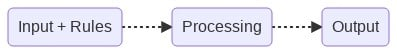
\includegraphics[width=0.7\textwidth]{classical.jpeg}
    \caption[Classical Programming]{Classical Programming}
    \label{fig:clsc_pgm}
\end{figure}

In machine learning the programmers supply the system with data and the expected output as input examples during training \cite{devto:urfstai}, as in figure \eqref{fig:mltrain}. During training period the machine improves in the tasks at hand gradually.

\begin{figure}[!htbp]
    \centering
    \begin{minipage}{0.45\textwidth}
        \centering
        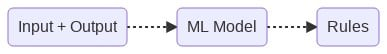
\includegraphics[width=1.1\textwidth]{ml_train.jpeg}
        \caption[ML Training]{\centering ML Training }
        \label{fig:mltrain}
    \end{minipage}\hfill
    \begin{minipage}{0.45\textwidth}
        \centering
        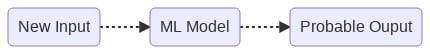
\includegraphics[width=1.1\textwidth]{ml_test.jpeg}
        \caption[ML Testing]{\centering ML Testing}
        \label{fig:mltest}
    \end{minipage}
\end{figure}

When the machine learning `model' is ready to map similar input output without humans explicitly defining each and every one of them, it enters the testing phase. The models is tested on some data which it has never seen before and predicts the output as shown in figure \eqref{fig:mltest}. There are various types of machine learning algorithms like: Supervised, Unsupervised adn Reinforced learning. Deep Learning is a subset of Machine Learning and it is called so because of the deep structure of the underlying architecture. 

\section*{Feed-forward Neural Networks}
\label{sec:ffnn}
\addcontentsline{toc}{section}{\nameref{sec:ffnn}}
\hspace{0.5cm} A feed-forward neural network is an artificial neural network wherein connections between the nodes do not form a cycle. The feed-forward neural network was the first and simplest type of artificial neural network devised. In this network, the information moves in only one direction—forward—from the input nodes, through the hidden nodes (if any) and to the output nodes. There are no cycles or loops in the network.

The simplest kind of neural network is a single-layer perceptron network, which consists of a single layer of output nodes; the inputs are fed directly to the outputs via a series of weights. The sum of the products of the weights and the inputs is calculated in each node, and if the value is above some threshold (typically 0) the neuron fires and takes the activated value (typically 1); otherwise it takes the deactivated value (typically -1) \cite{wiki:ffnn}. 

\section*{Activation Function}
\label{sec:actvfnc}
\addcontentsline{toc}{section}{\nameref{sec:actvfnc}}
In artificial neural networks, the activation function of a node defines the output of that node given an input or set of inputs. A standard integrated circuit can be seen as a digital network of activation functions that can be `ON' or `OFF', depending on input. A single-layer neural network can compute a continuous output instead of a step function. A common choice is the so-called logistic function:

\[f(x) = \frac{1}{1+e^{-x}}\]

The most common activation functions can be divided in three categories: ridge functions, radial functions and fold functions. Ridge functions are univariate functions acting on a linear combination of the input variables. Often used examples include, Linear: $\phi(v) = a + v'b$, ReLU $\phi(v) = max(0, a + v'b)$ etc. In multiclass classification the \emph{softmax} activation is often used \cite{wiki:actvfnc}.

\section*{Natural Language Processing}
\label{sec:nlp}
\addcontentsline{toc}{section}{\nameref{sec:nlp}}

Natural language processing (NLP) is concerned with the interactions between computers and human language, in particular how to program computers to process and analyze large amounts of natural language data. The result is a computer capable of ‘understanding’ the contents of documents, including the contextual nuances of the language within them. The technology can then accurately extract information and insights contained in the documents as well as categorize and organize the documents themselves.

Challenges in natural language processing frequently involve speech recognition, natural language understanding, and natural-language generation \cite{wiki:nlp}. 

\section*{Language Models}
\label{sec:langmodls}
\addcontentsline{toc}{section}{\nameref{sec:langmodls}}

\hspace{0.5cm} A statistical language model is a probability distribution over sequences of words. Given such a sequence, say of length $m$, it assigns a probability $P(w_1, \dots, w_m)$ to the whole sequence. The language model provides context to distinguish between words and phrases that sound similar. Data sparsity is a major problem in building language models. Most possible word sequences are not observed in \emph{training}. One solution is to make the assumption that the probability of a word only depends on the previous $n$ words. This is known as an $n$-gram model or unigram model when $n = 1$. The unigram model is also known as the \emph{bag of words model} \cite{wiki:langmdl}.

\section*{Transfer Learning}
\label{sec:trnsfrlrn}
\addcontentsline{toc}{section}{\nameref{sec:trnsfrlrn}}

\hspace{0.5cm} Transfer learning (TL) is a research problem in machine learning (ML) that focuses on storing knowledge gained while solving one problem and applying it to a different but related problem. For example, knowledge gained while learning to recognize cars could apply when trying to recognize trucks. This area of research bears some relation to the long history of psychological literature on transfer of learning.

From the practical standpoint, reusing or transferring information from previously learned tasks for the learning of new tasks has the potential to significantly improve the sample efficiency of a reinforcement learning agent. Given a source domain $D_S$ and learning task $T_S$, a target domain $D_T$ and learning task $T_T$, where $D_S \neq D_T$, or $T_S \neq T_T$, transfer learning aims to help improve the learning of the target predictive function $f_T(\cdot)$ in $T_T$ using the knowledge in $D_S$ and $T_S$ \cite{wiki:trnsflrn}.
\vspace*{\fill}

% !TeX root = ./seminar-report.tex
\chapter*{GPT-3 : Part 1 - The Transformer}
\label{chap:transformer}
\thispagestyle{fancy}
\addcontentsline{toc}{chapter}{\nameref{chap:transformer}}

\hspace{0.5cm} Introduced in 2017, The Transformer is a deep learning model primarily used in the field of natural language processing (NLP). Transformers are designed to handle sequential data, such as natural language unlike RNNs, Transformers do not require that the sequential data be processed in order. Thus Transformer allows for much more parallelization than RNNs and therefore reduced training hours. This has led to the development of pre-trained systems such as BERT (Bidirectional Encoder Representations from Transformers) and GPT (Generative Pre-trained Transformer), which have been trained with huge general language datasets, and can be fine-tuned to specific language tasks.

Transformer is an encoder-decoder architecture. The \emph{encoder} consists of a set of encoding layers that processes the input iteratively one layer after another and the \emph{decoder} consists of a set of decoding layers that does the same thing to the output of the encoder. Each encoder and decoder layer makes use of an \emph{attention mechanism}, which for each input, weighs the relevance of every other input and draws information from them accordingly to produce the output. Each decoder layer also has an additional attention mechanism which draws information from the outputs of previous decoders, before the decoder layer draws information from the encodings. Both the encoder and decoder layers have a feed-forward neural network for additional processing of the outputs, and contain residual connections and layer normalization steps \cite{wiki:transformer} as shown in figure \eqref{fig:trnsfrmarch}.

\begin{figure}[!htbp]
    \centering
    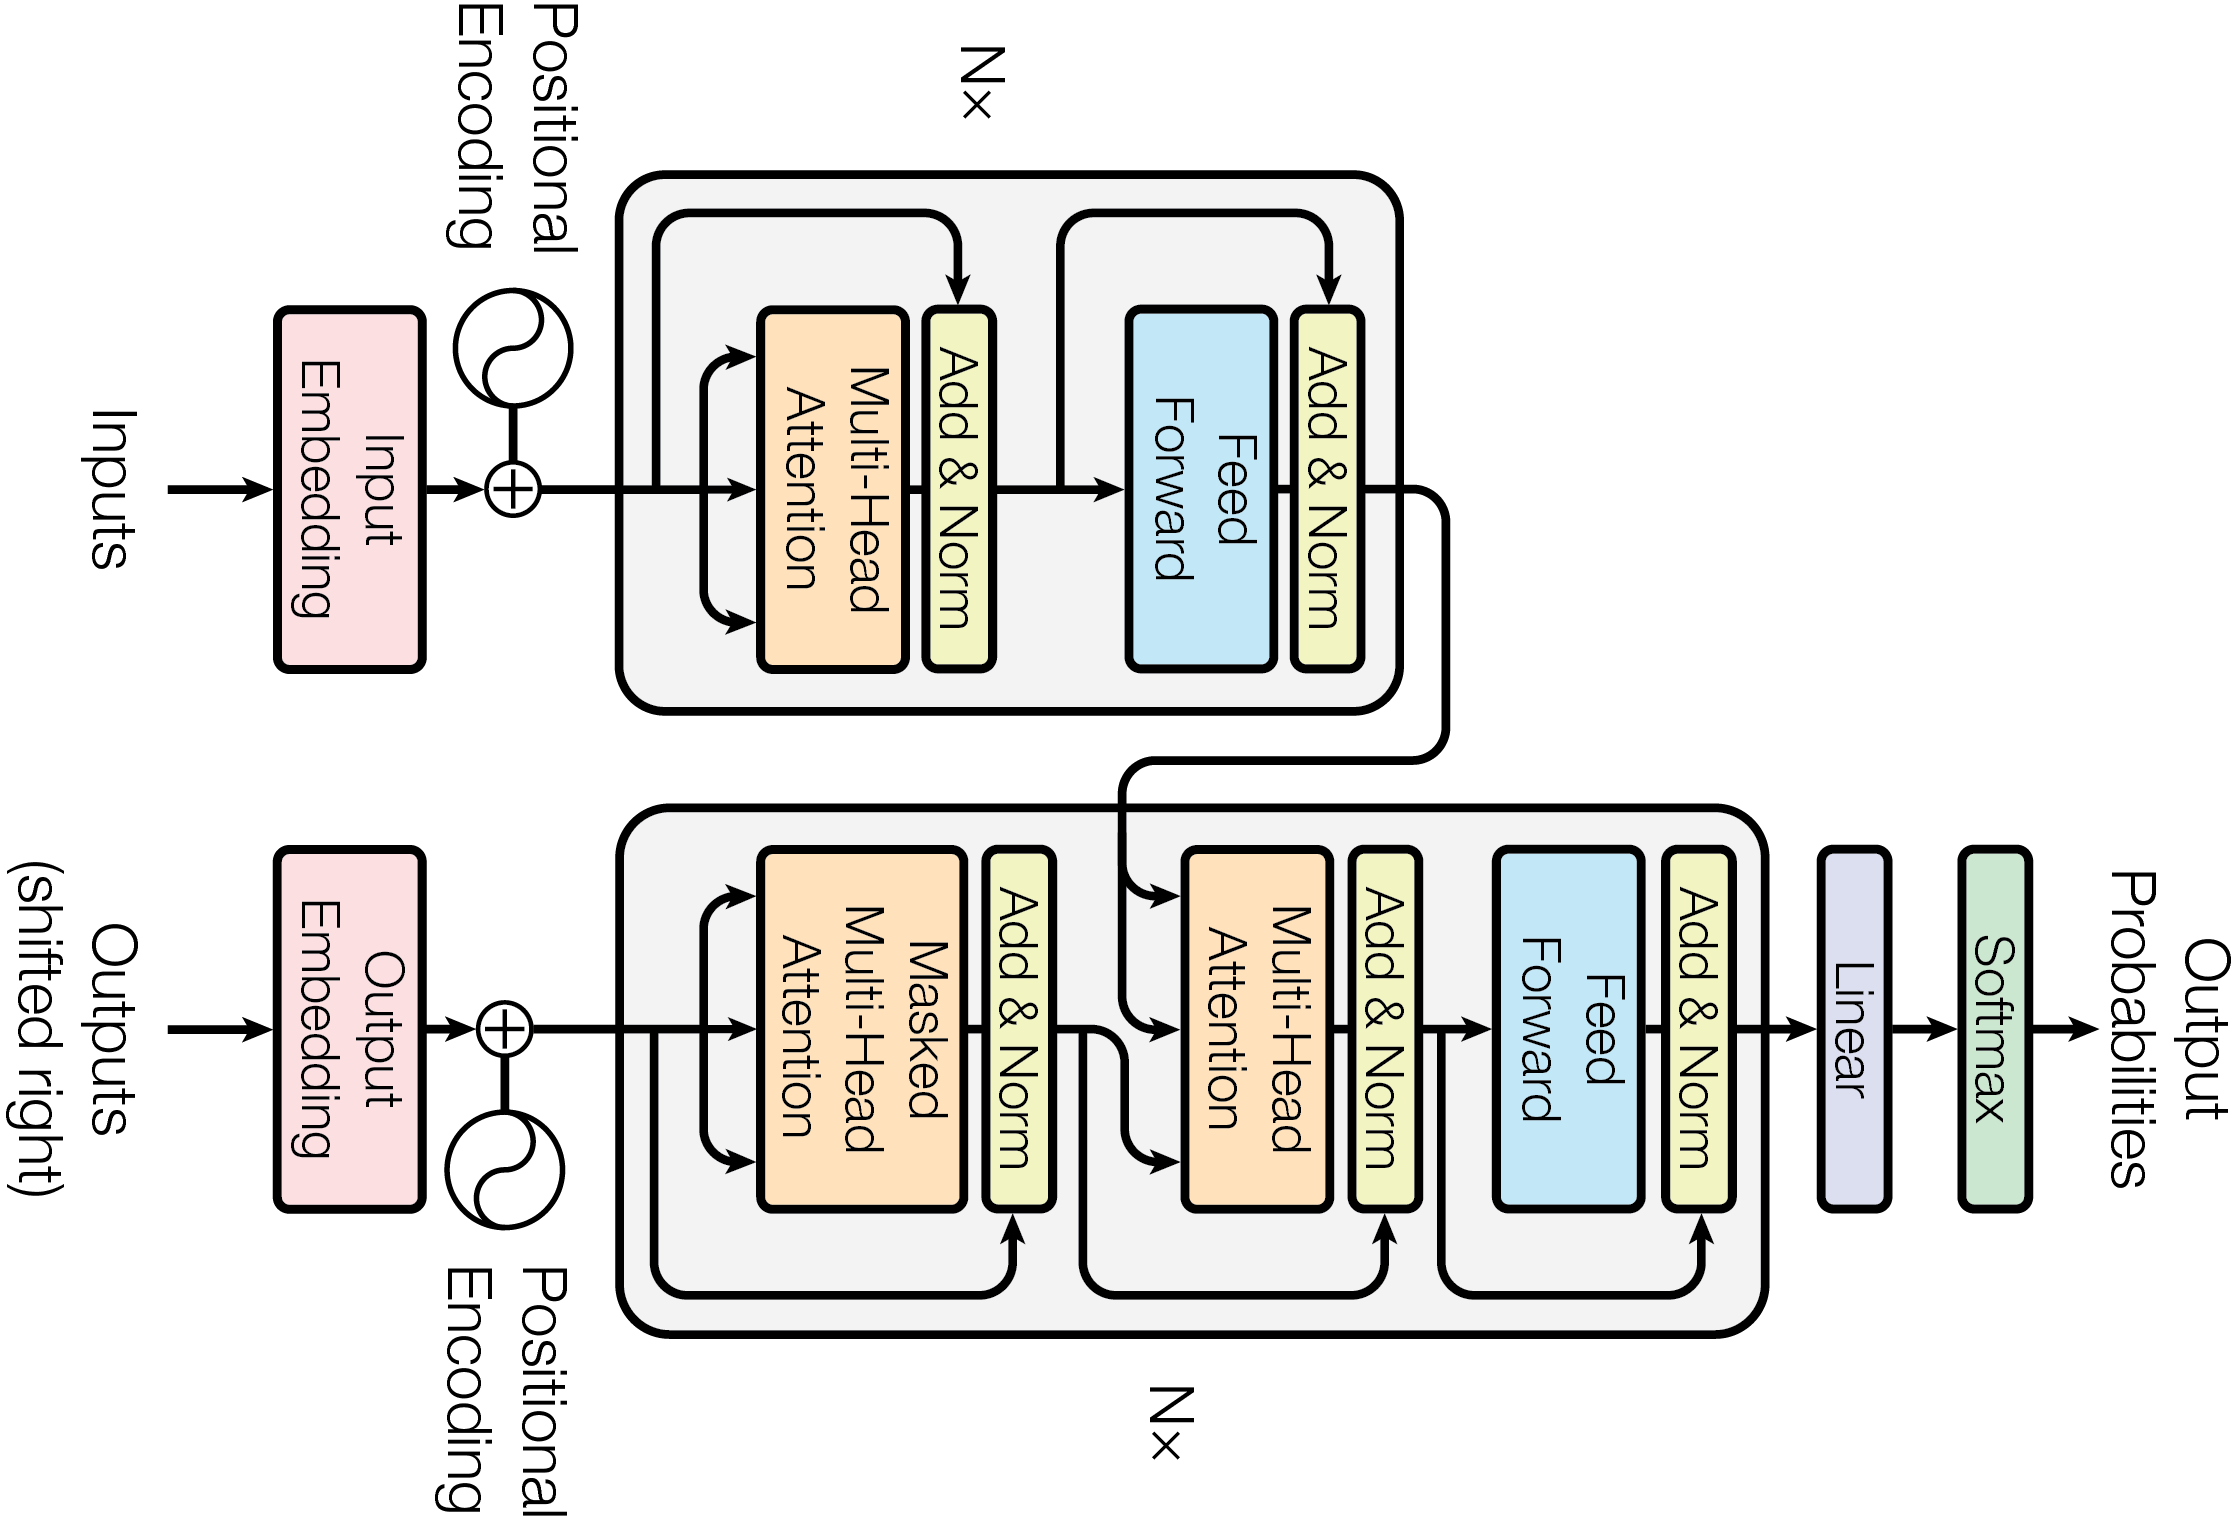
\includegraphics[width=0.7\textwidth]{transformer.png}
    \caption[The Transformer - model architecture]{The Transformer - model architecture \cite{2017arXiv170603762V}}
    \label{fig:trnsfrmarch}
\end{figure}

The basic building blocks of the Transformer are scaled dot-product attention units. When a sentence is passed into a Transformer model, attention weights are calculated between every token simultaneously. The attention unit produces embeddings for every token in context that contain information not only about the token itself, but also a weighted combination of other relevant tokens weighted by the attention weights.

\section*{Encoder}
\label{sec:encdr}
\addcontentsline{toc}{section}{\nameref{sec:encdr}}

\hspace{0.5cm} The encoder is composed of a stack of $N = 6$ identical layers. Each layer has two sub-layers. The first is a multi-head self-attention mechanism, and the second is a simple, position-wise fully connected feed-forward network. A residual connection \cite{2016arXiv160202410J} around each of the two sub-layers, followed by layer normalization \cite{2016arXiv160706450L}. That is, the output of each sub-layer is $LayerNorm(x + Sublayer(x))$, where $Sublayer(x)$ is the function implemented by the sub-layer itself. To facilitate these residual connections, all sub-layers in the model, as well as the embedding layers, produce outputs of dimension $d_{model} = 512$ \cite{2017arXiv170603762V}.

\section*{Decoder}
\label{sec:decdr}
\addcontentsline{toc}{section}{\nameref{sec:decdr}}

\hspace{0.5cm} The decoder is also composed of a stack of $N = 6$ identical layers. In addition to the two sub-layers in each encoder layer, the decoder inserts a third sub-layer, which performs multi-head attention over the output of the encoder stack. Similar to the encoder, residual connections are employed around each of the sub-layers, followed by layer normalization. The self-attention sublayer is also modified in the decoder stack to prevent positions from attending to subsequent positions. This masking, combined with fact that the output embeddings are offset by one position, ensures that the predictions for position $i$ can depend only on the known outputs at positions less than $i$ \cite{2017arXiv170603762V}.

\section*{Attention Mechanism}
\label{sec:attnmec}
\addcontentsline{toc}{section}{\nameref{sec:attnmec}}

\hspace{0.5cm} An attention function can be described as mapping a query and a set of key-value pairs to an output, where the query, keys, values, and output are all vectors. The output is computed as a weighted sum of the values, where the weight assigned to each value is computed by a compatibility function of the query with the corresponding key.

The input consists of queries and keys of dimension $d_k$, and values of dimension $d_v$. The dot products of the query with all keys is computed then each one divided by $\sqrt{d_k}$. Finally a \emph{softmax} function is applied to obtain the weights on the values. In practice, the attention function on a set of queries is computed simultaneously, packed together into a matrix $Q$. The keys and values are also packed together into matrices $K$ and $V$ as shown in figures \eqref{fig:sdpa} and \eqref{fig:mmha}. The matrix of outputs is computed as \cite{2017arXiv170603762V}:

\[\textnormal{Attention}(Q, K, V) = \textnormal{softmax}(\frac{(Q K^T)}{\sqrt{d_k}})V\]

The two most commonly used attention functions are additive attention \cite{2014arXiv14090473B}, and dot-product (multiplicative) attention. Dot-product attention is identical to our algorithm, except for the scaling factor of $\frac{1}{\sqrt{d_k}}$ . Additive attention computes the compatibility function using a feed-forward network with a single hidden layer. Dot-product attention is much faster and more space-efficient in practice, since it can be implemented using highly optimized matrix multiplication code.

\begin{figure}[!htbp]
    \centering
    \begin{minipage}{0.45\textwidth}
        \centering
        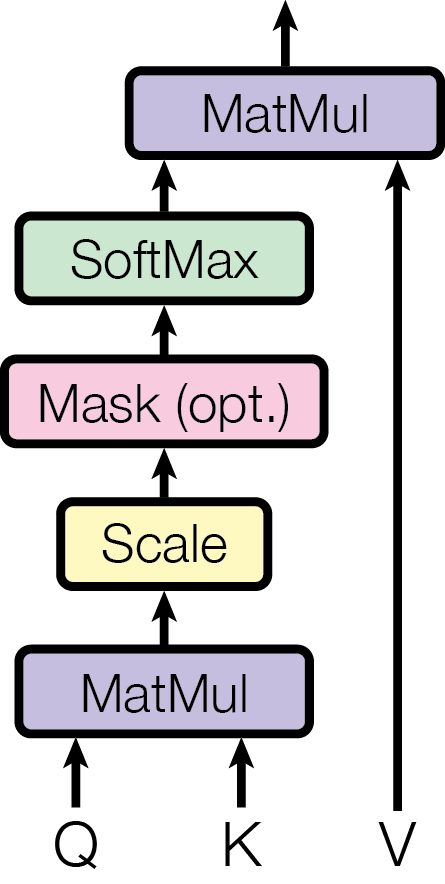
\includegraphics[height=0.7\textwidth]{scaled_dot_attention.png}
        \caption[Scaled Dot-Product Attention]{\centering Scaled Dot-Product Attention \cite{2017arXiv170603762V}}
        \label{fig:sdpa}
    \end{minipage}\hfill
    \begin{minipage}{0.45\textwidth}
        \centering
        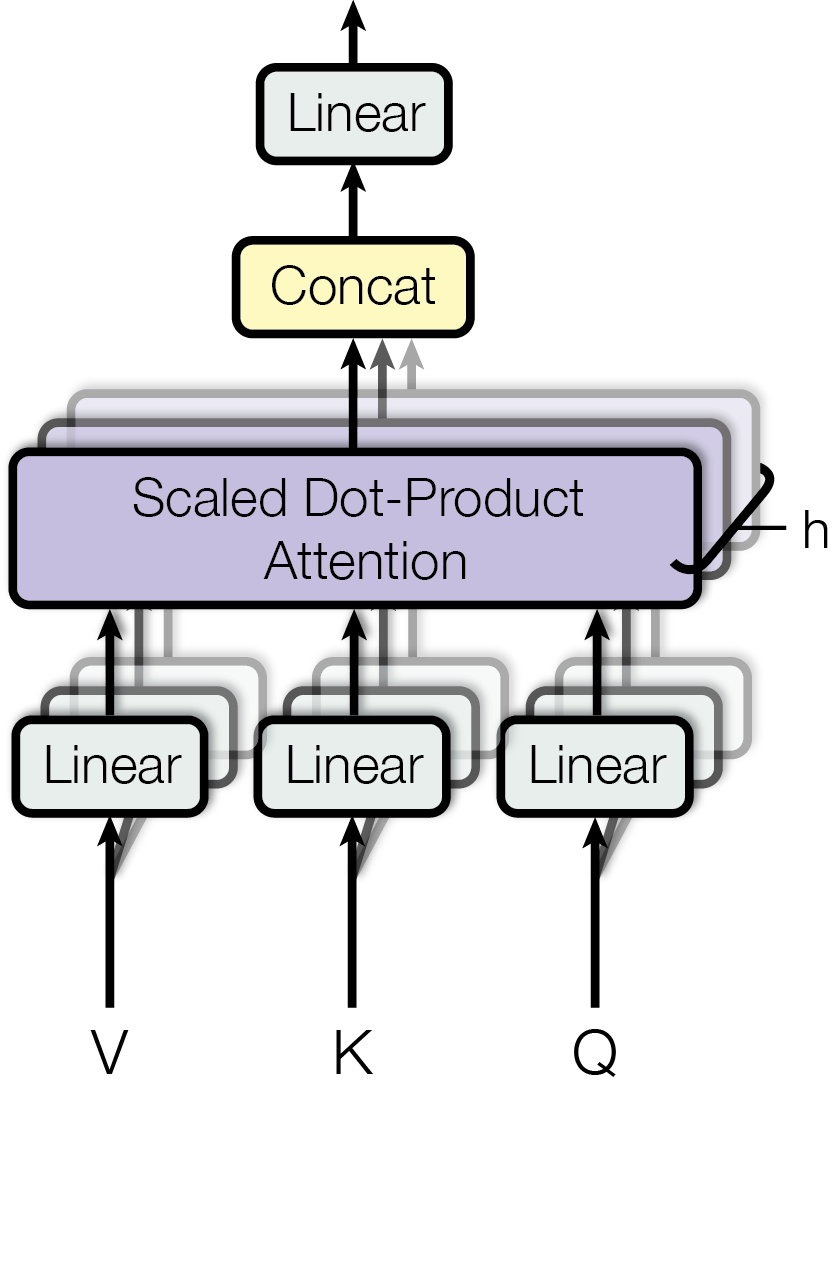
\includegraphics[height=0.7\textwidth]{masked_multihead_attention.png}
        \caption[Masked Multi-head Attention]{\centering Masked Multi-head Attention \cite{2017arXiv170603762V}}
        \label{fig:mmha}
    \end{minipage}
\end{figure}

While for small values of $d_k$ the two mechanisms perform similarly, additive attention outperforms
dot product attention without scaling for larger values of $d_k$ \cite{2017arXiv170303906B}. For large values of $d_k$, the dot products might grow large in magnitude, pushing the \emph{softmax} function into regions where it has extremely small gradients. To counteract this probable effect, the dot products is scaled by $\frac{1}{\sqrt{d_k}}$ \cite{2017arXiv170603762V}.

\section*{Multi-Head Attention}
\label{sec:mlthdatn}
\addcontentsline{toc}{section}{\nameref{sec:mlthdatn}}

\hspace{0.5cm} Instead of performing a single attention function with $d_{model}$ - dimensional keys, values and queries, it was found that it's beneficial to linearly project the queries, keys and values $h$ times with different, learned linear projections to $d_k$ , $d_k$ and $d_v$ dimensions, respectively. On each of these projected versions of queries, keys and values the attention function was performed in parallel, yielding $d_v$ - dimensional output values. These are concatenated and once again projected, resulting in the final values, as depicted in figure \eqref{fig:mmha}.

Multi-head attention allows the model to jointly attend to information from different representation
subspaces at different positions. With a single attention head, averaging inhibits this.

\[\textnormal{MultiHead}(Q, K, V) = \textnormal{Concat(head}_1, \hdots, \textnormal{head}_\textnormal{h})W^O \]
\[\textnormal{where head}_\textnormal{i} = \textnormal{Attention}(QW_i^Q, KW_i^K, VW_i^V)\]

Where the projections are parameter matrices $W_i^Q \in \mathbb{R}^{d_{model}\times d_k}$, $W_i^V \in \mathbb{R}^{d_{model}\times d_v}$ and $W^O \in \mathbb{R}^{hd_v\times d_{model}}$ \cite{2017arXiv170603762V}.

\vspace*{\fill}

\chapter*{GPT-3 : Part 2 - Demonstration}
\label{chap:demonstration}
\thispagestyle{fancy}
\addcontentsline{toc}{chapter}{\nameref{chap:demonstration}}
\vspace*{\fill}

\chapter*{GPT-3 : Part 3 - Issues and Critiques}
\label{chap:critiques}
\thispagestyle{fancy}
\addcontentsline{toc}{chapter}{\nameref{chap:critiques}}
\vspace*{\fill}

\chapter*{Conclusion}
\label{chap:conclusion}
\thispagestyle{fancy}
\addcontentsline{toc}{chapter}{\nameref{chap:conclusion}}
\vspace*{\fill}

\bibliographystyle{unsrt}
\bibliography{references}
\thispagestyle{fancy}

\end{document}